% !TeX spellcheck = en_EN-English

\section{Record Cost Prediction}
\label{recCostPred}

Next step in total cost prediction is to predict how much each record would cost. For this we choose standard multilayer perceptron (MLP) or in another words multi-layered fully-connected feed-forward neural network. 

\subsection{Multilayer perceptron}
\label{MLP}

Multilayer perceptron is a feed-forward neural network, so network where data flow single direction or in other words neurons don't form cycles. This network consist of fully-connected, sometimes called dense, layers with non-linear activation functions as shown on Fig. \ref{fig:mlp}, where we can see that this model can be split into three parts which are input layer which load the data, hidden layer which are trying to extract desired information using linear transformations and activation functions and finally output layer which contains final linear transformation followed by activation to output extracted information. Each layer can be described using this formula:

\begin{equation}
	\label{eqn:mlp}
	h_i = act(W_i h_{i-1} + b_i),
\end{equation}
where $h_i$ is resulting vector of i-th layer, $act()$ is a non-linear activation function, $W_i$ is weight matrix of i-th layer, $h_{i-1}$ is resulting vector from previous layer and $b_i$ is bias vector.

\begin{figure}[!h]
	\centering
	
	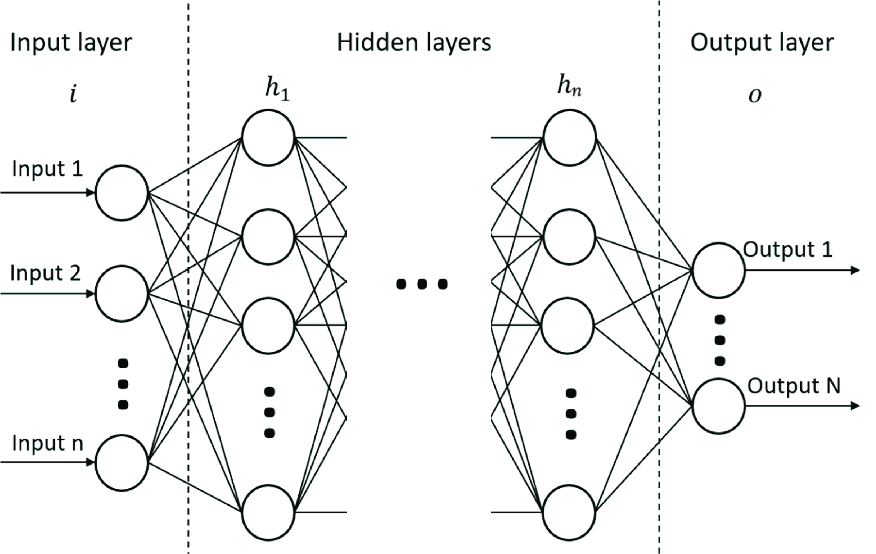
\includegraphics[width=0.8\textwidth]{images/MLP_arch.png}
	
	\caption{Architecture of multilayer perceptron \cite{MLParch}}
	\label{fig:mlp}
\end{figure} 